\documentclass[varwidth, border=0pt]{standalone}

\usepackage{times}      % Loads the Times-Roman Fonts
\usepackage{mathptmx}   % Loads the Times-Roman Math Fonts
\usepackage{subcaption}
\usepackage[labelfont={bf,sf},%
labelsep=period,%
justification=centering,
labelformat=parens,labelsep=quad,skip=3pt,font=scriptsize]{caption}
\usepackage{graphicx}
\usepackage{multicol}

\begin{document}
	
	\begin{figure}
	\centering
\begin{subfigure}{\linewidth}
	\begin{multicols}{2}
		\centering
		\begin{subfigure}{\linewidth}
			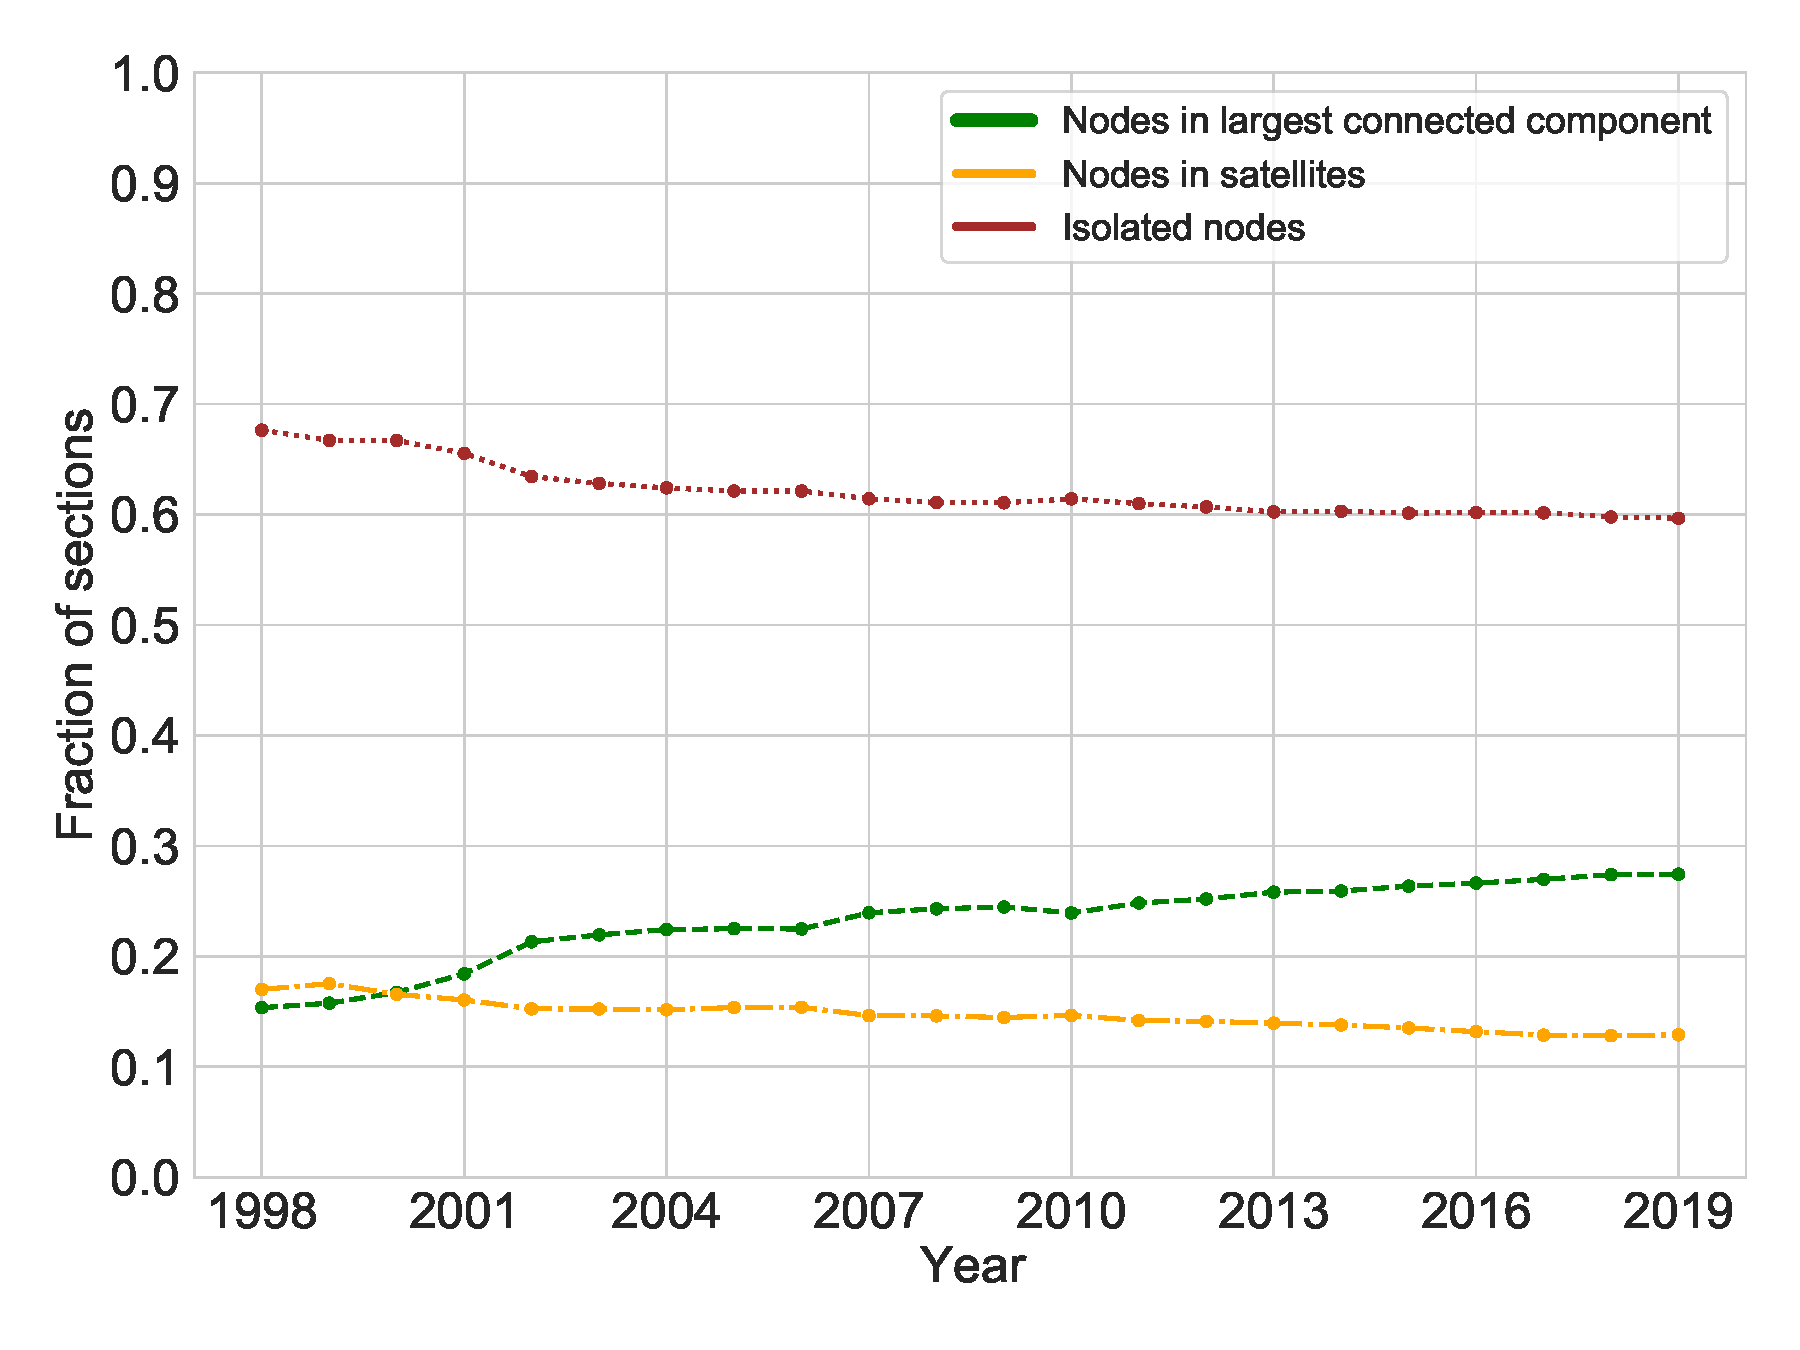
\includegraphics[width=\linewidth]{../../graphics/connectivity-development-regulations-only-us.pdf}
			\caption*{\textbf{\textsf{(i)}}\quad Overall}
		\end{subfigure}
		\newpage
		\begin{subfigure}{\linewidth}
			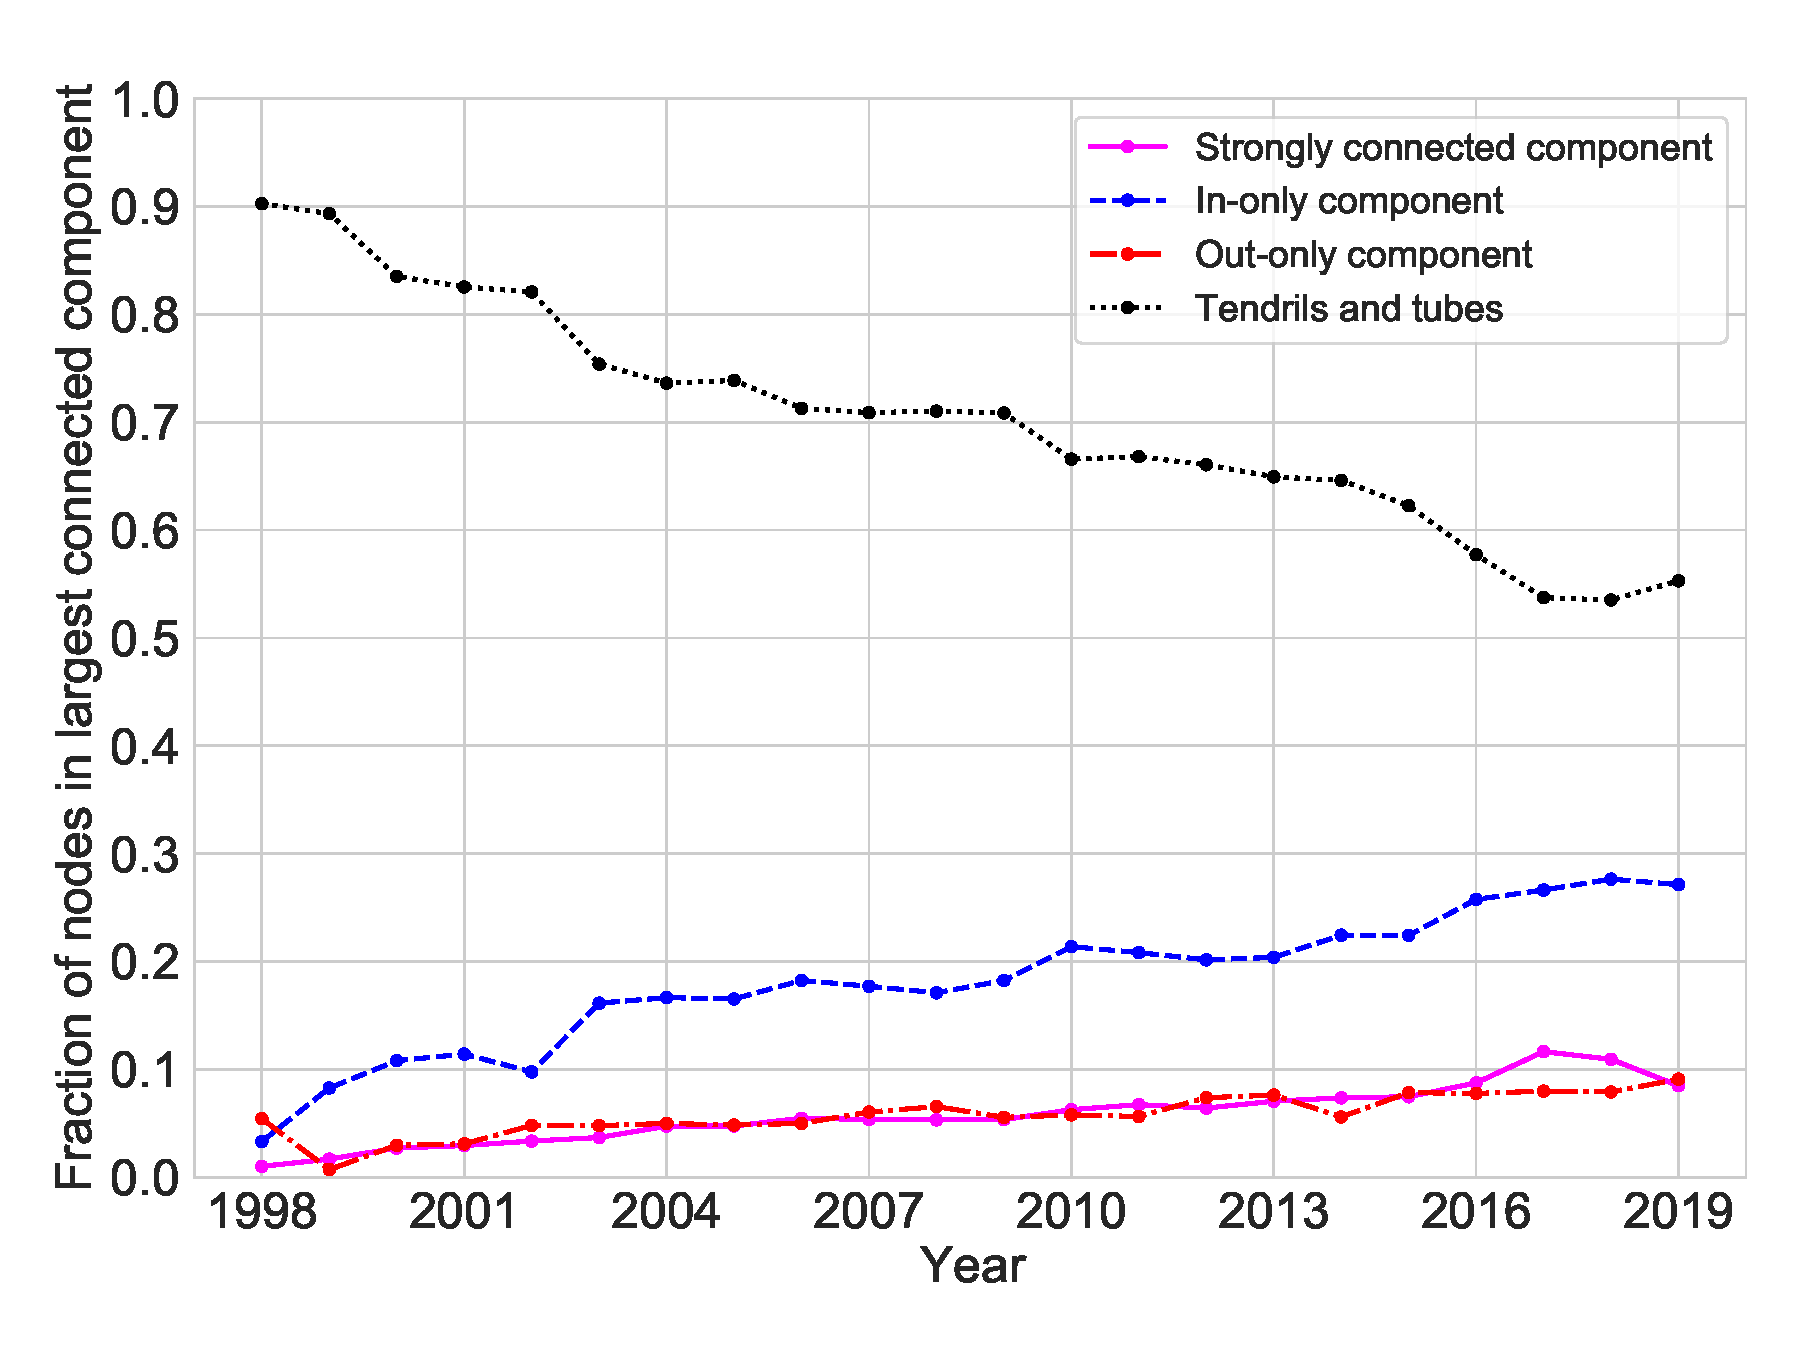
\includegraphics[width=\linewidth]{../../graphics/connectivity-lcc-regulations-only-us.pdf}
			\caption*{\textbf{\textsf{(ii)}}\quad Largest Connected Component}
		\end{subfigure}	
	\end{multicols}
	\vspace*{-6pt}\subcaption{United States}
\end{subfigure}

\vspace*{6pt}

\begin{subfigure}{\linewidth}
	\begin{multicols}{2}
		\centering
		\begin{subfigure}{\linewidth}
			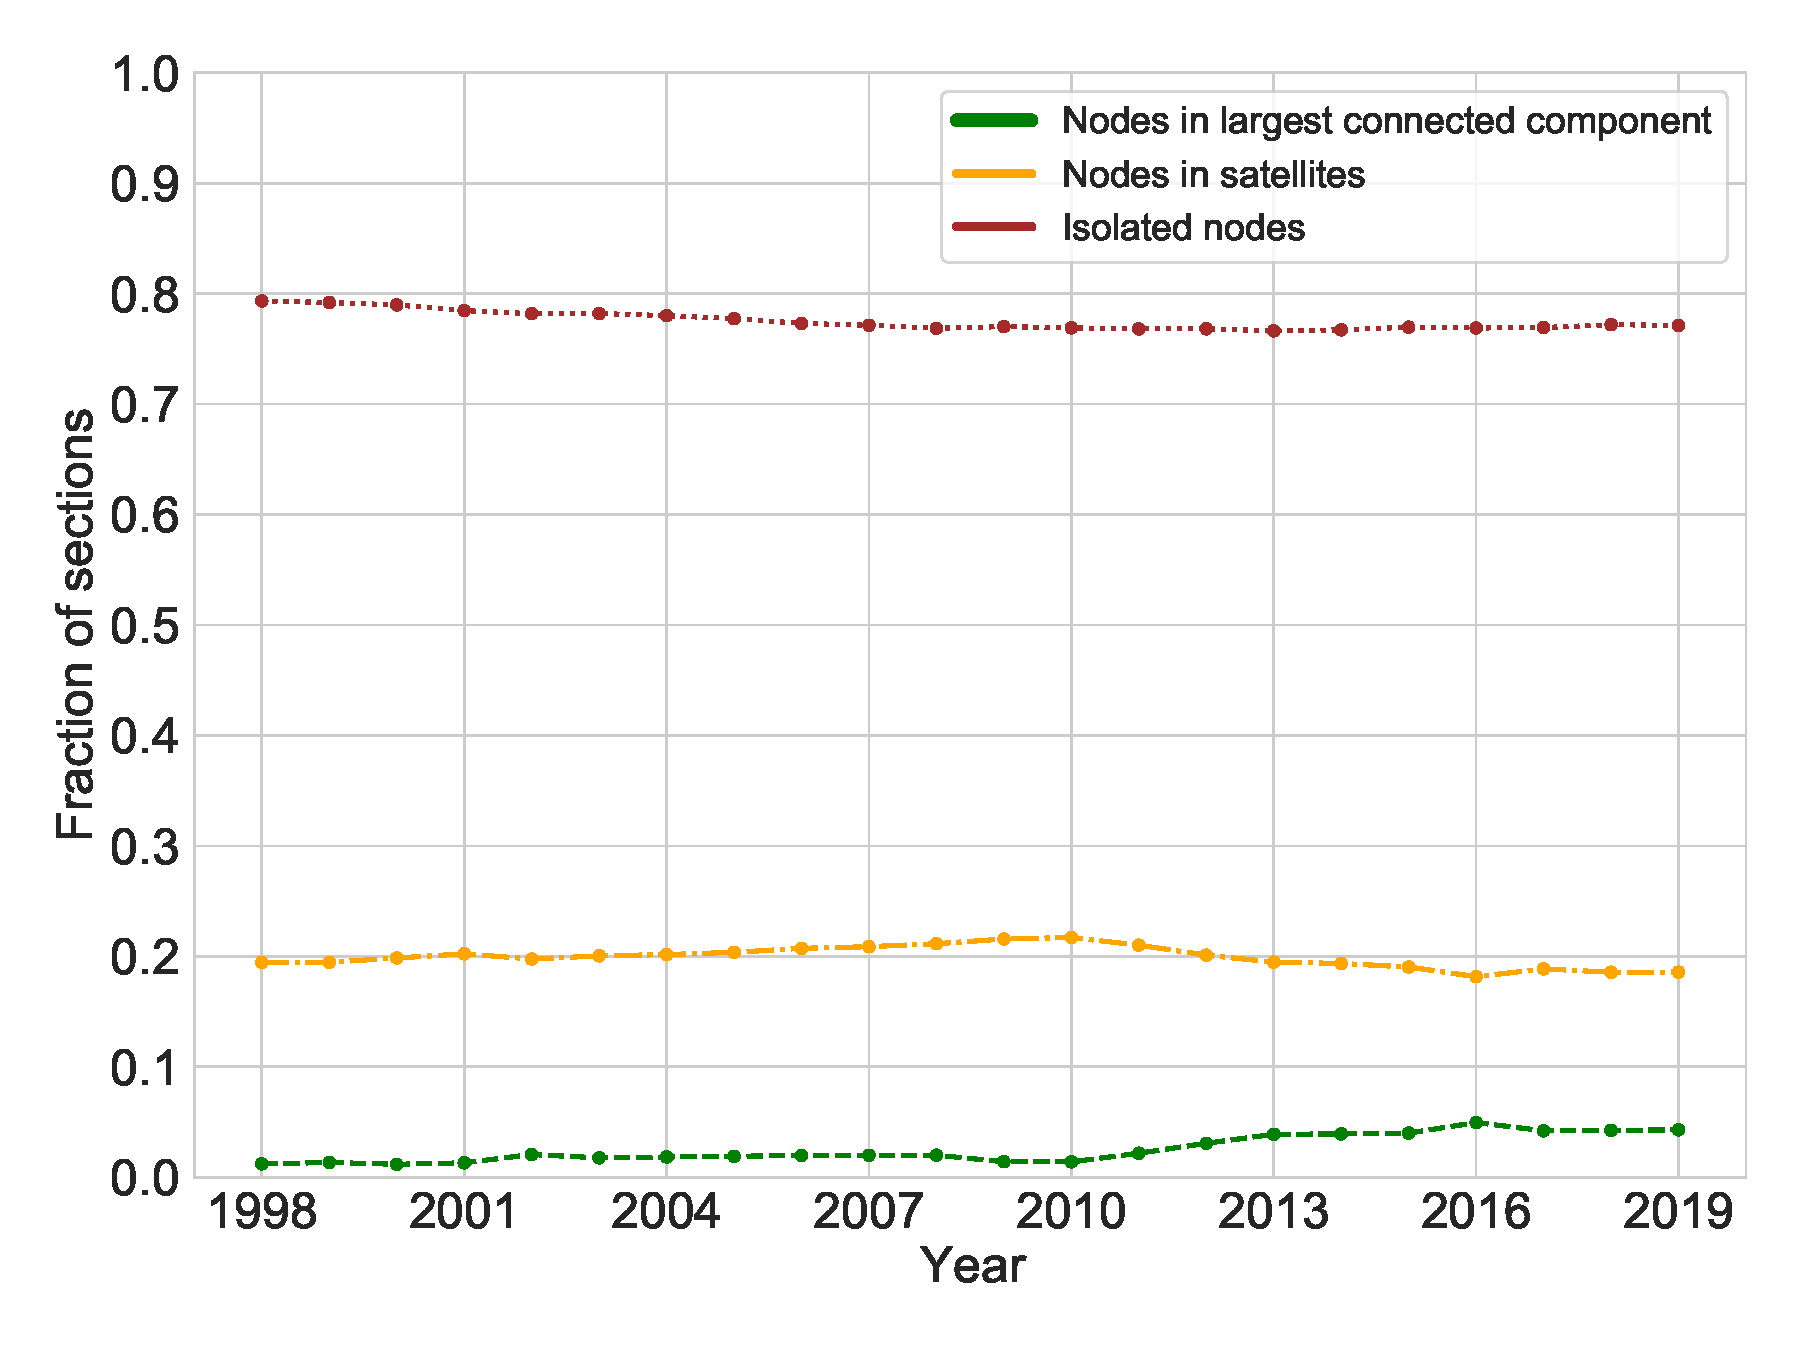
\includegraphics[width=\linewidth]{../../graphics/connectivity-development-regulations-only-de.pdf}
			\caption*{\textbf{\textsf{(i)}}\quad Overall}
		\end{subfigure}
		\newpage
		\begin{subfigure}{\linewidth}
			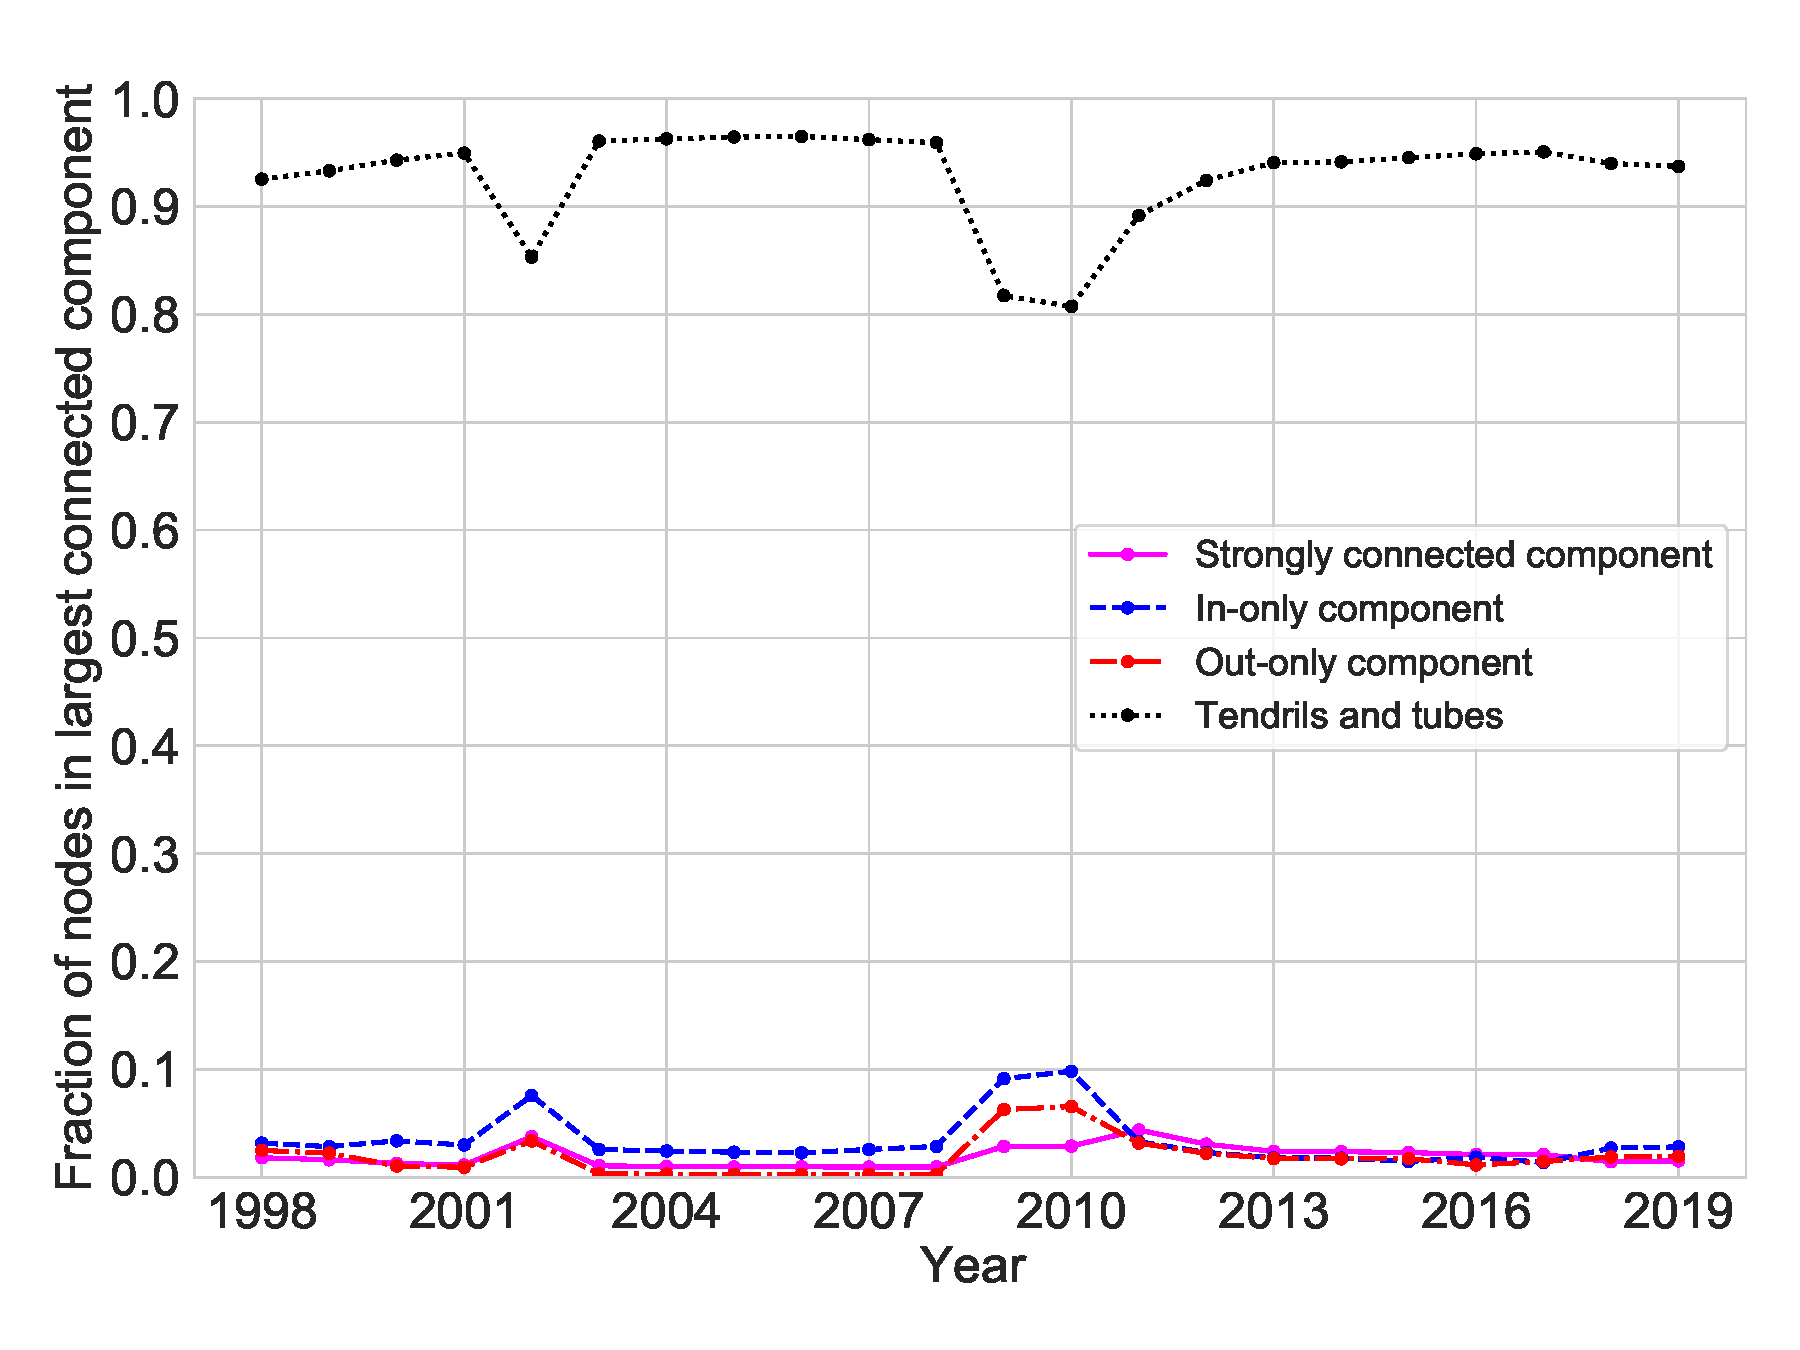
\includegraphics[width=\linewidth]{../../graphics/connectivity-lcc-regulations-only-de.pdf}
			\caption*{\textbf{\textsf{(ii)}}\quad Largest Connected Component}
		\end{subfigure}	
	\end{multicols}
	\vspace*{-6pt}\subcaption{Germany}
\end{subfigure}
	\end{figure}
	
\end{document}